\documentclass{standalone}
\usepackage{tikz}
\usepackage{amsmath}
\usepackage{units}
\begin{document}
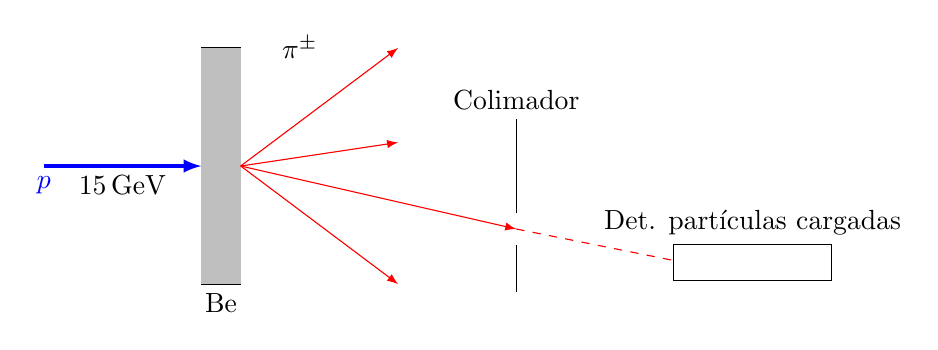
\begin{tikzpicture}
   %Lámina de Berilio
   \draw[] (0,1.5) rectangle (0.5,-1.5);
   \fill[lightgray] (0,1.5) rectangle (0.5,-1.5);
   \node[below] at(0.25,-1.5){Be};
    % Trazo de partículas
    \draw[very thick,blue,-latex] (-2,0)node[below]{$p$} -- (0,0);
    \node[below] at(-1,0){$\unit[15]{GeV}$};
    \draw[-latex,red] (0.5,0)--(2.5,1.5);
    \draw[-latex,red] (0.5,0)--(2.5,0.3);
    \draw[-latex,red] (0.5,0)--(4,-0.8);
    \draw[-latex,red] (0.5,0)--(2.5,-1.5);
    \node at((1.25,1.5){$\pi^\pm$};
    %Colimador
    \draw[] (4,-0.6)--(4,0.6) node[above]{Colimador};
    \draw[] (4,-1)--(4,-1.6);
    
    \draw[dashed,red] (4,-0.8)--(6,-1.2);
    \draw[] (6,-1.45) rectangle(8,-1);
    \node[above] at(7,-1){Det. partículas cargadas};
\end{tikzpicture}
\end{document}